\documentclass{article}

\usepackage{fullpage}
\usepackage{graphicx}
\usepackage{amsfonts, amsmath}
\usepackage{url}
\usepackage{hyperref}
\usepackage{float}
\usepackage[final]{pdfpages}

\hypersetup{
	colorlinks=true,
	linkcolor=black
}

\begin{document}

\clearpage
\vspace*{\stretch{2}}
\begin{center}
\begin{minipage}{.6\textwidth}

\title{Automatic ``Music'' Generator \\ \vspace{2 pt} \text{Final Report}}
\author{Sam Fleckenstein (sef44) \\ Ross Nanopoulos (rdn21)}
\maketitle

\end{minipage}
\end{center}
\vspace{\stretch{3}}
\clearpage

\tableofcontents
\newpage

\section{Abstract}
The purpose of this project is to develop an intelligent music composer that will analyze common and popular patterns in music, reason about those patterns, and generate a new piece of music that is significantly different than the analyzed pieces, while still being interesting.

\newpage

\section{Introduction}
What is the process by which humans make music? They study the fundamentals: beats, measures, time and key signatures, tempo, rhythm. They listen to great composers: Bach, Tchaichovsky, Mahler, Debussy, Chopin. Somehow this knowledge combined with creativity yields additional, masterful compositions. How then, does one enable a computer to exhibit this thoughtful creativity?\\
\\
A variety of methods have been proposed for algorithmic composition including hidden Markov models \cite{5492670}, genetic algorithms \cite{514161}, and neural networks \cite{4667040}. Additionally, a field known as "combination theory" has combined these methods to create more advanced learning and composition algorithms \cite{4626654}. Hidden Markov Models utilize an element of probability and uncertainty that can lead to much more interesting compositions
\\
The argument can be made that innate creativity plays a large role in being able to compose interest- ing music. However, a goal of artificial intelligence is to eventually develop systems that can think and have personalities of their own. Thus, this innate creativity when composing music will develop with more advanced artificially intelligent systems that can think for themselves and exhibit such behavior.

\section{Application}
\subsection{The Echo Nest Interface}
The backbone of the Echo Nest interface will be The Echo Nest’s large database of music intelligence. The song parser will utilize The Echo Nest’s API to extract useful song information from the database, which includes a plethora of aspects including time signature, key, mode, tempo, loudness, duration, end of fade in, start of fade out, audio fingerprint, timbre, pitch, and loudness. Additionally, The Echo Nest provides sequenced data as ”musically relevant elements” that include segments, tatums, beats, bars, and sections.  This information will allow the learning agent to discern the myriad dynamics of songs and learn about the ways in which different songs are composed.

\subsection{Learning Agent}
The job of the learning agent will be to take the raw music data gathered by Echo Nest and discover the relevant patterns in the music. There are a number of different algorithms that could be used to achieve this goal, but this project uses a hierarchical hidden Markov model to extract these patterns. A hierarchical hidden Markov model is a generalization of hidden Markov models, where each state is itself a hidden Markov Model. \cite{Fine:1998:HHM:325865.325879} This allows the learning agent to utilize the inherent structure of music to provide a more informed model.\\
\\
Additionally, hierarchical hidden Markov models have been used to look at pitch structure in music.   \cite{_learningmusical} In relation to this project, the learning agent looks at the patterns within the higher structure of the music in the Echo Nest's sections (i.e. patterns of choruses, verses, bridges, etc.). Then it moves deeper into the next level of musical events, bars, and continues this process all the way down to the level of notes, where the respective hidden Markov model will learn the actual sequence of pitches and duration of these notes. 

This model was chosen because it can be used to represent processes where not all of the information about a state is known. This is useful because music is very complex and it is very difficult to determine every variable that goes into determining what should come next in a song. Another reason that hidden Markov models were chosen for this project is because they have been successfully applied the automatic generation of music \cite{5492670}. The complexity of a hidden Markov model is also very easy to expand. This can be done by looking at data that is farther in the past from the current observation, or by adding in more variables to the states being considered. Finally, the hierarchical structure of hidden Markov models allows the learning agent to best utilize the structure of the Echo Nest's data, which has the many levels of structure inherent to music.

\subsection{Composition Agent}
The composition agent will take the information that the learning agent provides and decide which notes, patterns, rhythms, etc. to incorporate into its own piece of music. It will then be responsible for outputting this generated music to a .wav file, which can be used later for further analysis and classification.

\section{Methodology}
\subsection{The Echo Nest Interface}
This interface utilizes pyechonest, a python wrapper for The Echo Nest's Main API, in order to collect an audio summary, which contains the basic information for a song such as the key, mode, tempo, time signature, and an analysis URL (i.e. where the sequenced data for each song lives). The sequenced datea can be easily accessed via The Echo Nest's Remix API; therefore, this interface only needs to pass a list of track IDs to the learning agent.

\subsection{Learning Agent}
The learning agent utilizes the GHMM library to perform the required machine learning on the patterns of sequenced data for which the user rates highly. A hidden Markov model was created for each level of musical events, as specified by The Echo Nest's API. These musical events include, from largest to smallest: sections, bars, beats, tatums, and segments. Currently, the learning agent learns from all of the musical events separately; however, the next phase of development will focus on recursively moving down the structure of the music, and then reconstructing the song from the bottom upwards.

\section{Software Design}
\subsection{User Interface}
\begin{enumerate}
\item The UI will prompt the user for a musical genre (COMPLETED)
\item The UI will prompt the user for a song tempo (COMPLETED)
\item The UI will prompt the user for a time signature (COMPLETED)
\item The UI will prompt the user for a key signature (COMPLETED)
\item The UI will send user choices to the Echo Nest Interface (COMPLETED)
\end{enumerate}

\subsection{The Echo Nest Interface}
\begin{enumerate}
\item The Echo Nest Interface will take as input the user input from the UI (COMPLETED)
\item The Echo Nest Interface will make a call to The Echo Nest API using the user input (COMPLETED)
\item The Echo nest will provide a list of track IDs to be utilized by the learning agent (COMPLETED)
\end{enumerate}

\subsection{User Feedback}
\begin{enumerate}
\item The user will be prompted to rate a number of short song clips (IN PROGRESS)
\item The user ratings will be tabulated and used to update the learned model based on which musical patterns the user rated highest
\item The user will be presented with one longer song based on the updated musical model
\item The user feedback will be injected to the relevant stages of the hierarchical hidden Markov model to improve the learning
\end{enumerate}

\subsection{Learning Agent}
\begin{enumerate}
\item The learning agent will use the GHMM library
\item The learning agent will take as input track IDs from the Echo Nest interface (COMPLETED)
\item The learning agent will utilize The Echo Nest's Remix API \cite{Remix} to access sequenced data from track IDs (COMPLETED)
\item The learning agent will train a model using the GHMM library and the input from the Echo Nest Interface 
\item The learning agent will output a trained model to the composition agent 
\end{enumerate}

\subsection{Composition Agent}
\begin{enumerate}
\item The composition agent will take as input a trained model from the learning agent (COMPLETED)
\item The composition agent will create a sequence of sections from the model
\item The composition agent will create a sequence of bars from the model as it relates to sections
\item The composition agent will create a sequence of beats from the model as it relates to bars
\item The composition agent will create a sequence of tatums from the model as it relates to beats
\item The composition agent will create a sequence of segments as it relates to tatums
\item The composition agent will write the resulting composition to disk as a .wav file (IN PROGRESS)
\end{enumerate}

\section{Project Management}
\subsection{Communication}
In order to facilitate on-time delivery of the Intelligent Music Generator, in-person meetings 
will be held at least once at week on Thursdays at 4:30. In addition to this, meetings will be 
held as necessary to discuss upcoming deadlines as well as any issues that have come up. 
Communication will also happen during the rest of the week primarily via email.


\subsection{Source Control}
Github will be used for feature tracking and reporting bugs.  Pull requests will be utilized to 
ensure that each member has reviewed the code before it enters the master branch.  Branches will 
be utilized for implementing different components and features.

\subsection{Work Division}
The work division will be as follows. Ross will be reponsible for the primary development and 
implementaiton of the HHMM in the learning agent. Sam will be responsible for the design and 
implementation of the composition agent. Both members will utilize the various APIs provided by
The Echo Nest to complete their tasks.  This is not a hard division of the work as each of 
the group members will also be working a great deal on the parts of the project they are not in
charge of. This division of work fits well with the strengths and experience of each of the 
project members.

\subsection{Management Plan Effectiveness}
The largest issue with the management plan has been changes to the learning agent. These changes have necessitated a pushback of the timeline for the learning agent. This has not been too large of an issue because other work that does not rely on the learning agent has continued while the learning agent has been delayed. Given this, the project should still complete on time.\\
\\
The communication method has been an effective way of keeping on track to complete assigned tasks.  It has also allowed questions to be asked more frequently, so that getting stuck on one particular challenge for too long is not an issue.\\
\\
In regards to version control, when the project started, merging commits were a problem due to constantly changing and moving parts. This has been resolved, however, and merging has become a much smoother process.\\
\\
As such, the project management plan will be kept largely the same, except for shifting around of when various parts of the project will occur.

\subsection{Now to the End}
Given the changes that have been made to the learning agent, timelines have been pushed back. The project should still finish on time, but it may not be as well polished as is desirable.
\\
During the next stage of the project, the focus will be shifting towards completing the learning agent, and towards implementing the composition agent. Since various components of the project are getting finished up, they will also be hooked together to form a more functional product.

Lastly, much of the code is currently repetitive between the different musical event learners. There is discussion about creating a hidden Markov model state factory class that will be able to be passed the type of musical event (section, beat, segment, etc.), the alphabet for that type (chorus verse bridge, a e a d, etc.), as well as the respective transmission and emission matrices. This factory will create the hidden Markov model states that will be utilized by the learning agent.

\section{User Interface}
The user interface will be implemented as a web application. First the user will be prompted to choose a genre, tempo, time signature, and key signature.  The user will click begin, and will be played short sound clips, which can be rated 1 to 4 (this will be updated to words, once it is decided which will provide a better user experience).  After the default number of music clips, the user can choose to rate more music clips or compose a song.  Below are screen shots of the application flow:

\Large{TODO: fill in the new UI} \normalsize

\section{Testing and Evaluation}
The testing is currently all manual. Each of the developers is responsible for testing all of their
components to make sure that they work properly, but the present focus of the project is the 
implementation of all required features. Once all of the desired features are implemented, a
more thorough testing procedure will be implemented to ensure the music generator works as designed.

\section{Lessons Learned}
\subsection{The Echo Nest Interface}

\subsection{Learning Agent}
The largest problem with the learning agent was what information the learning was based off of. At the beginning of the project, it was thought that looking at the group of previous notes would give enough information to guess what the next note should be. The design of the learning agent was based around this assumption, which turned out to be a fatal flaw.\\
\\
After the program got to the point where it was first outputting "music", several different methods were implemented to see if the subjective quality of the output could be improved. First, the number of previous notes examined was increased an decreased, with no noticeable change in musical quality. The next attempt was to try splitting up pitches and durations. The learning agent initially learned based in tuples of pitch and duration values because it was thought that each of these values could potentially influence the other. After splitting these two up, there was also no dicernible change in the quality of the music. One benefit this provided, however, was a major decrease in the runtime of the program.\\
\\
Before this change was implemented, the program was taking about 900 seconds to execute end to end. This included gathering data on what songs the user was interested in, learning off of those songs, and then generating the music. The most unfortunate part about this stage of the project was that the learning agent was only looking at a single song during those 900 seconds. Because about 75\% of the execution time was in an external library, there was almost nothing we could do about this issue.\\
\\
After separating the pitches from the durations, the learning agent had a much smaller set of possible values to look at, which resulted in a runtime of about 70 seconds to learn from a single song. This is still rather slower than is optimal because the initial plan was to have the learning agent look at a large number of songs, possibly in the range of 100.\\
\\
Were this project to continue, a major redesign of the learning agent would be the first step. It seems that in order for the learning agent to be able to learn anything useful about the music it is presented, the agent would need to have much more knowledge of how music is composed. Instead of simply looking at notes and durations, the agent could be programmed to look for specific patterns in the music that extend beyond just notes.\\
\\
At this time, that sort of knowledge is not available to either of the team members, which means that some sort of expert on musical composition would most likely have to be found and added to the team. With the knowledge of someone who is experienced in composing, it would be possible to implement a much more intelligent learning agent.

\subsection{Composition Agent}

\subsection{User Interface}


\section{Discussion}

\newpage

\section{Appendices}
\subsection{Database Design}
As there is not a large quantity of data to be saved for this project, there is no associated 
database.

\subsection{User Manual}

\subsection{Programmer Manual}

\newpage

\bibliography{References}
\bibliographystyle{plain}

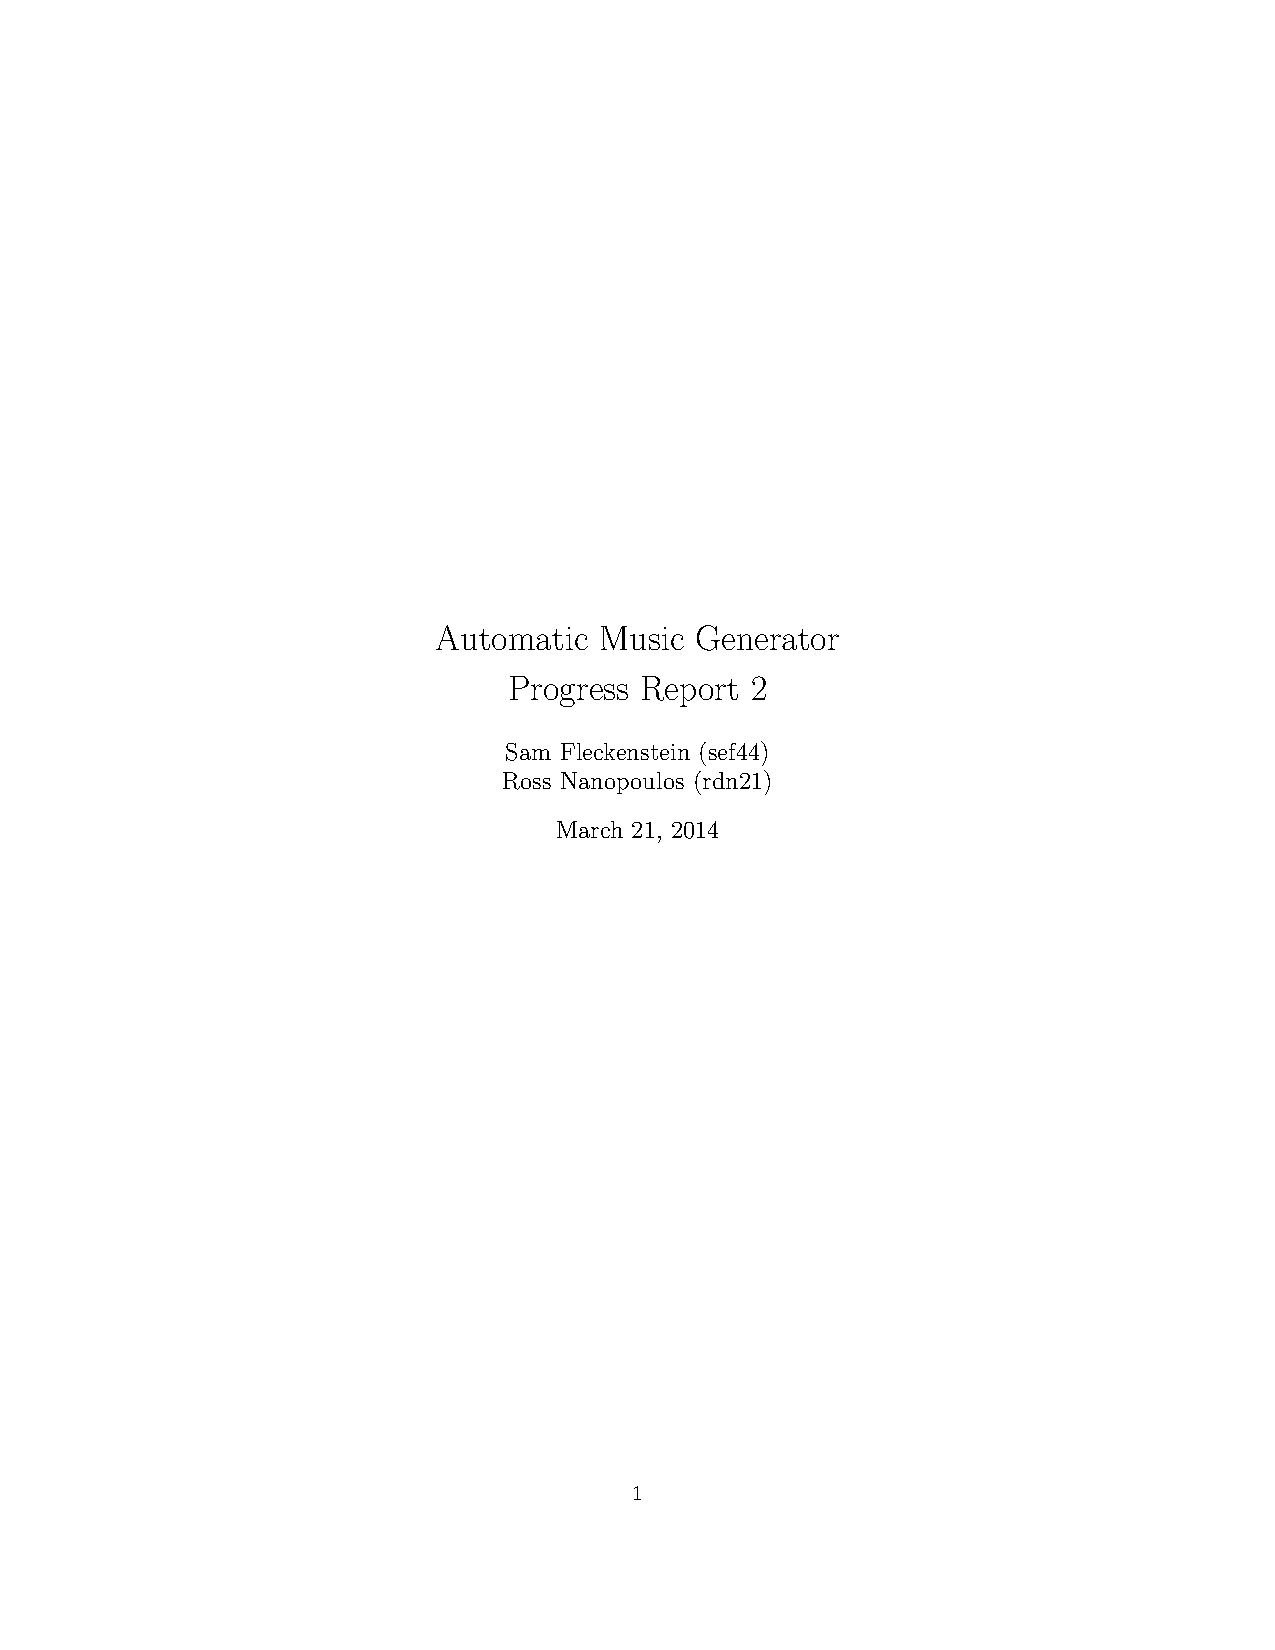
\includepdf[pages=-]{ProgressReport2.pdf}

\end{document}
